\documentclass[10pt,a4paper,final]{report}
\usepackage[utf8]{inputenc}
\usepackage[english]{babel}

%reasonable borders
\setlength{\hoffset}{-1.8cm} 
\setlength{\voffset}{-2cm}
\setlength{\textheight}{24.0cm} 
\setlength{\textwidth}{17cm}

\usepackage[T1]{fontenc}
\usepackage{tgpagella}
\usepackage{cmap}
\usepackage[plainpages=false,pdfpagelabels,unicode]{hyperref}

\usepackage{pdfpages}
\usepackage[pdftex]{color}
\usepackage{graphicx}

\usepackage{url}
\usepackage[toc]{appendix}


%\usepackage{amsmath}
%\usepackage{amsfonts}
%\usepackage{amssymb}
%\usepackage{graphicx}

\usepackage{color}
\usepackage{listings}
\lstset{ %
language=bash,                % choose the language of the code
basicstyle=\footnotesize,       % the size of the fonts that are used for the code
%numbers=left,                   % where to put the line-numbers
%numberstyle=\footnotesize,      % the size of the fonts that are used for the line-numbers
%stepnumber=1,                   % the step between two line-numbers. If it is 1 each line will be numbered
%numbersep=5pt,                  % how far the line-numbers are from the code
%backgroundcolor=\color{white},  % choose the background color. You must add \usepackage{color}
showspaces=false,               % show spaces adding particular underscores
showstringspaces=false,         % underline spaces within strings
showtabs=false,                 % show tabs within strings adding particular underscores
frame=single,   		% adds a frame around the code
columns=flexible,
keepspaces=true,
tabsize=4,  		% sets default tabsize to 2 spaces
%captionpos=b,   		% sets the caption-position to bottom
breaklines=true,    	% sets automatic line breaking
breakatwhitespace=true,    % sets if automatic breaks should only happen at whitespace
%escapeinside={\%}{)}          % if you want to add a comment within your code
}

%\makeatletter
%\def\lst@filenamerpl{_\textunderscore $\textdollar --\- -\-}
%\makeatother
%\lstset{columns=flexible}
%\lstset{keepspaces=true}
%\lstset{showspaces=true}
%\makeatletter
%\def\lst@visiblespace{\textcolor{codebg}{-}}
%\makeatother
%\makeatletter
%\def\lst@outputspace{{\ifx\lst@bkgcolor\empty\color{white}\else\lst@bkgcolor\fi\lst@visiblespace}}
%\makeatother

\author{Lukáš Bezdička}
\title{Nagios to Splunk}
\begin{document}

\setcounter{page}{1}
\pagenumbering{roman}

\chapter*{Abstract}
This work tries to explore Nagios and Splunk integration. Idea is to monitor several machines with Nagios and report changes in their state to Splunk, allowing not only reporting of the incidents but also analysis on larger scale. Splunk could provide trend prediction which is Nagios lacking at the moment.\footnote{\url{http://en.wikipedia.org/wiki/Comparison\_of\_network\_monitoring\_systems}}
\section*{Nagios}
Nagios is an open-source infrastructure monitoring system. It's used to alert system administrators about problems, usually before they are noticed by the end user. This is achieved by periodical checks of resources through Nagios plugins. Nagios already has a huge database of available plugins and offers well documented API for writing new ones.\footnote{\url{http://nagios.sourceforge.net/docs/3\_0/pluginapi.html}}
\section*{Splunk}
Splunk is an enterprise software used to monitor, report and analyze the machine data produced by the applications, systems and infrastructure that run a business. Splunk lets users search, monitor and analyze machine-generated data via web-style interface. Splunk captures indexes and correlates real-time data in a searchable repository from which it can generate graphs, reports, alerts and dashboards.\footnote{\url{https://secure.wikimedia.org/wikipedia/en/wiki/Splunk}}
\newpage

\setcounter{tocdepth}{3}
\setcounter{page}{1}
\pagenumbering{arabic}

\tableofcontents

\chapter{Theory and Setup}
The chosen architecture is best described by picture [\ref{NtS}]. Checks on particular hosts are performed by running scripts invoked from nrpe\footnote{Nagios Remote Plugin Executor - \url{http://nagios.sourceforge.net/docs/3\_0/addons.html}}, via ssh or by snmpd. For each of these there is a Nagios plugin, namely check\_by\_nrpe, check\_by\_ssh and check\_snmp\_extend. Nagios determines the status of a host or service by evaluating the return code from plugins. These are:
\begin{figure}[hbpt]
\begin{center}
\begin{tabular}{|c|c|c|}
\hline Return code & Service state & Host state \\ 
\hline 0 & OK & UP \\ 
\hline 1 & WARNING & Up or DOWN/UNREACHABLE\footnote{\url{http://nagios.sourceforge.net/docs/3\_0/networkreachability.html}} \\ 
\hline 2 & CRITICAL & DOWN/UNREACHABLE \\ 
\hline 3 & UNKNOWN & DOWN/UNREACHABLE \\ 
\hline 
\end{tabular}
\end{center}
\caption{Nagios plugin return codes and corresponding service or host states.}
\label{ReturnC}
\end{figure}

Nagios logs every host or service state change and depending on configuration sends alerts. It's logs then can be forwarded to Splunk to be indexed. Connected with other data in Splunk this can provide ways to analyze trends on vast systems. 

\begin{figure}[hbpt]
\begin{center}
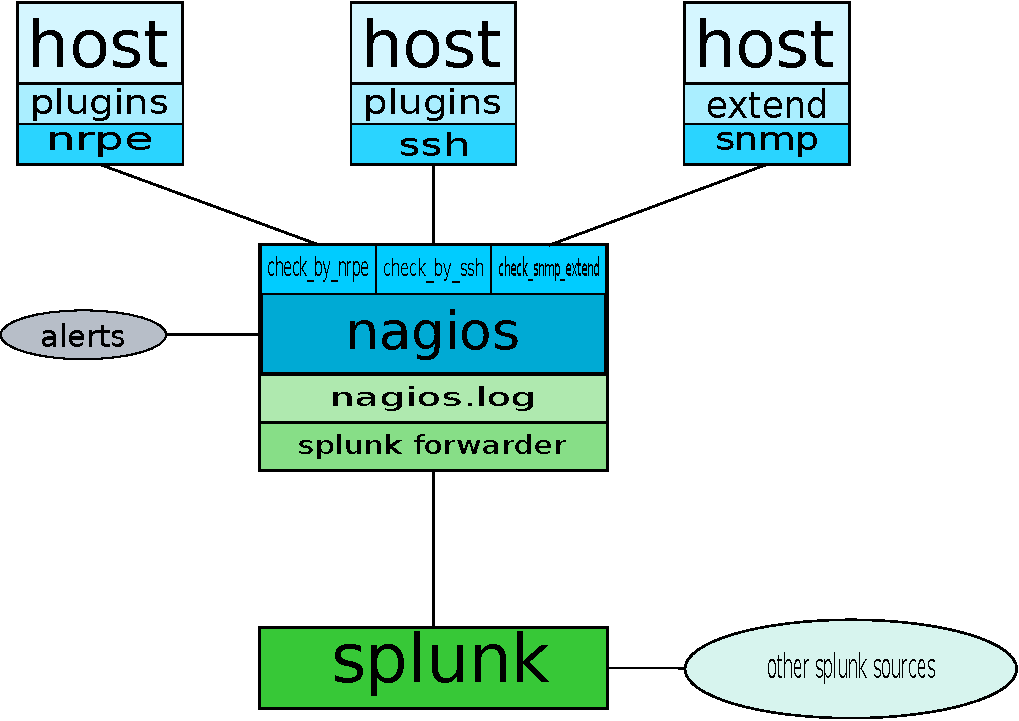
\includegraphics[scale=0.5]{nts.pdf}
\end{center}
\caption{Nagios to Splunk}
\label{NtS}
\end{figure}

The actual setup consisted of:
\begin{itemize}
\item VM - Splunk: Running splunkd and recieving data from other sources.
\item VM - Nagios: Running nagios and collecting data through NRPE on Splunk and Hypervisor.
\item VMM - AthenA: Running virtual machines and generating at least some interesting data for Nagios and Splunk.
\end{itemize}
Operating systems used were Fedora 15 for hypervisor and Scientific Linux 6.1 for virtual machines, so this process should be similar or same on all of the latest RedHat-like systems.

\section{Hypervisor}
Required packages for virtualization with KVM:
\begin{lstlisting}
yum install libvirt qemu-kvm virt-manager virt-viewer dhcp
\end{lstlisting} 
Fedora 12 adds KSM (Kernel SamePage Merging) which allows identical memory pages to be merged by the kernel into a single page. This is especially useful for KVM when running multiple guests from the same or similar base operating system image.\footnote{\url{http://fedoraproject.org/wiki/Features/KSM}} To enable KSM just run:

\begin{lstlisting}
chkcofig ksm on
systemctl start ksm.service
chkcofig ksmtuned on
systemctl start ksmtuned.service
\end{lstlisting}
The KSM is enabled by default but sharing only 2000 pages. By starting \emph{ksm} service you can share up to half of system's memory. To control and tune \emph{ksm} there is \emph{ksmtuned} daemon with configuration in \emph{/etc/ksmtuned.conf}.\footnote{\url{http://docs.redhat.com/docs/en-US/Red\_Hat\_Enterprise\_Linux/6/html/Virtualization/chap-KSM.html}}

Virtual Machine Manager has quite straightforward GUI, so only note about network, as I wanted to use dhcp to configure hostnames and ips, just disable dhcp for virtual network and setup \emph{dhcpd}:

\begin{lstlisting}
#/etc/dhcp/dhcpd.conf
##option definitions common to all supported networks...
option domain-name-servers 192.168.1.1;
ddns-update-style none;
#ddns-rev-domainname "in-addr.arpa";

authoritative;

default-lease-time 600;
max-lease-time 7200;

subnet 192.168.100.0 netmask 255.255.255.0 {
  range 192.168.100.100 192.168.100.254;
  option routers 192.168.100.1;
}


host nagios {
  option host-name "nagios";
  hardware ethernet 52:54:00:53:44:f2;
  fixed-address 192.168.100.20;
}

host splunk {
  option host-name "spluk";
  hardware ethernet 52:54:00:a2:66:9f;
  fixed-address 192.168.100.10;
}
\end{lstlisting}
And start \emph{dhcpd}:
\begin{lstlisting}
chkconfig dhcpd on
systemctl start dhcpd.service
\end{lstlisting}

\section{Virtual Machines}
Default minimal install of SL6.1 is quite sufficient and depending on setup only few packages are required which are listed in later sections. It shouldn't be hard to create kickstart file or pupet configuration. Only additional steps are to add repositories for these packages:
\begin{lstlisting}
yum install http://download.fedora.redhat.com/pub/epel/6/i386/epel-release-6-5.noarch.rpm
\end{lstlisting}
%Update might be broken because of *-logos packages so update with:
%\begin{lstlisting}
%yum --skip-broken update
%\end{lstlisting}
\subsection{VM images}
Small note about offline work with VMs, when you can't or don't want to run them, but just want to work with the files, use:
\begin{lstlisting}
losetup /dev/loop1 /home/social/libvirt/images/Nagios.img #or other location of your .img
kpartx -a /dev/loop1
# default on RHlike systems is to use lvm so:
pvscan
vgchange -ay
mount /dev/VolGroup/lv_root /mnt/
\end{lstlisting}
And close them:
\begin{lstlisting}
umount /dev/VolGroup/lv_root
vgchange -an
kpartx -d /dev/loop1
losetup -d /dev/loop1
\end{lstlisting}

\chapter{Nagios}

Setting up Nagios can get quite complex and actual setup may vary based on real size and state of network. In this case we'll create templates for three types of hosts depending on way they are going to be checked. To get Nagios running you need to install \emph{httpd} and \emph{php} and for ssl you need \emph{mod\_ssl}:
\begin{lstlisting}
yum install nagios nagios-plugins nagios-devel httpd mod_ssl php nagios-plugins-ping nagios-plugins-http nagios-plugins-ssh
\end{lstlisting}
Change \emph{ServerName} directive in \emph{/etc/httpd/conf/httpd.conf} to corresponding ip.
Edit \emph{/etc/httpd/conf.d/nagios.conf}, leave "\emph{Allow from all}" but enable "\emph{SSLRequireSSL}" for security reasons. Start \emph{httpd} daemon:
\begin{lstlisting}
chkconfig httpd on
service httpd start
chkconfig nagios on # already configure start on boot
\end{lstlisting}
Web interface configuration is located in \emph{/etc/nagios/cgi.cfg}. To allow \emph{guest} login add \emph{authorized\_for\_read\_only=guest}. You can also enable integration functionality with Splunk here by adding:
\begin{lstlisting}
enable_splunk_integration=1
splunk_url=http://<host>:<port>/en-US/app/search/flashtimeline
\end{lstlisting}
Where \emph{<host>} stands for ip or hostname and \emph{<port>} is port of web interface (usually 8000). This way you'll be presented with "Splunk It" links in various places in the web interface.
\newline Setup passwords for \emph{nagiosadmin}, \emph{guest}:
\begin{lstlisting}
htpasswd -c /etc/nagios/passwd nagiosadmin 
htpasswd /etc/nagios/passwd guest
\end{lstlisting}
%novy riadok dost jebe odseky TODO zmazat
The main configuration file \emph{/etc/nagios/nagios.cfg} is basically self-explanatory with the comments inside of it. So only few notes: 
\begin{itemize}
\item \emph{log\_file=/var/log/nagios/nagios.log} will be used later for splunk\_forwarder.
\item \emph{cfg\_file} and \emph{cfg\_dir} specify object configuration files or directories to scan for configuration files.
\item set \emph{check\_external\_commands=1} in order to allow commands to be executed from the web interface.
\end{itemize}
External commands file will probably have broken access rights, to fix this:
\begin{lstlisting}
chown nagios:apache /var/spool/nagios/cmd/nagios.cmd
\end{lstlisting}
Basic configuration in \emph{nagios.conf} should contain:
\begin{lstlisting}
# OBJECT CONFIGURATION FILE(S)
# These are the object configuration files in which you define hosts,
# host groups, contacts, contact groups, services, etc.
# You can split your object definitions across several config files
# if you wish (as shown below), or keep them all in a single config file.

cfg_file=/etc/nagios/objects/commands.cfg
cfg_file=/etc/nagios/objects/contacts.cfg
cfg_file=/etc/nagios/objects/timeperiods.cfg
cfg_file=/etc/nagios/objects/templates.cfg
cfg_file=/etc/nagios/objects/contactgroups.cfg
\end{lstlisting}
Don't forget to open 443 port for https in iptables and start \emph{nagios} service.

\section{Objects}
Objects are all the elements that are involved in the monitoring and notification logic. In other words there is basic set of object types which you can configure in flexible template format, allowing object inheritance to create and manage complex configurations.\footnote{\url{http://nagios.sourceforge.net/docs/3\_0/objectdefinitions.html}} Basic object types are:
\begin{itemize}
\item Hosts - usually represent physical devices e.g. servers, workstations, routers, switches, printers, etc. You can define their addresses, services and relations.
\item Host Groups - groups of related hosts to simplify configuration and view of their status on web interface.
\item Services - represent all services associated with host like attributes (load,uptime,etc), services provided by host (http,ssh,etc.) and services related to host (DNS,etc.).
\item Service Groups - similar to host groups.
\item Contacts - define all the people involved in notification process and their notification methods.
\item Contact Groups - simplify configuration of all the people involved with certain hosts.
\item Timeperiods - time periods definitions for monitoring and alerting.
\item Commands - definitions of programs and scripts to perform when doing checks.
\end{itemize}

\subsection{\emph{timeperiods.cfg}}
Example of \emph{/etc/nagios/objects/timeperiods.cfg}:
\begin{lstlisting}
define timeperiod{
        timeperiod_name 24x7
        alias           24 Hours A Day, 7 Days A Week
        sunday          00:00-24:00
        monday          00:00-24:00
        tuesday         00:00-24:00
        wednesday       00:00-24:00
        thursday        00:00-24:00
        friday          00:00-24:00
        saturday        00:00-24:00
        }
# 'czech_holidays'  timeperiod definition with Easter for 2012~2017
define timeperiod{
		name			czech_holidays
        timeperiod_name czech_holidays
        alias           Czech holidays
        january 1       00:00-00:00 ; Den obnovy samostatneho ceskeho statu
        may 8           00:00-00:00 ; Den osvobozeni
        july 5          00:00-00:00 ; Den slovanskych verozvestu Cyrila a Metodeje
        july 6          00:00-00:00 ; Den upaleni mistra Jana Husa (first czech cosmonaut)
        september 28    00:00-00:00 ; Den ceske statnosti
        october 28      00:00-00:00 ; Den vzniku samostatneho ceskoslovenskeho statu
        november 17     00:00-00:00 ; Den boje za svobodu a demokracii
        january 1       00:00-00:00 ; Novy rok
        may 1           00:00-00:00 ; Svatek prace
        december 24 - 26    00:00-00:00 ; Vanoce
        2012-04-09      00:00-00:00 ; Velikonocni pondeli 2012
        2013-04-01      00:00-00:00 ; Velikonocni pondeli 2013
        2014-04-21      00:00-00:00 ; Velikonocni pondeli 2014
        2015-04-06      00:00-00:00 ; Velikonocni pondeli 2015
        2016-03-28      00:00-00:00 ; Velikonocni pondeli 2016
        2017-04-17      00:00-00:00 ; Velikonocni pondeli 2017	
        }
# 'workhours' timeperiod definition with czech_holidays
define timeperiod{
        timeperiod_name workhours
        use				czech_holidays
        alias           "Normal" Working Hours
        monday          08:00-17:00
        tuesday         08:00-17:00
        wednesday       08:00-17:00
        thursday        08:00-17:00
        friday          08:00-17:00
        }
# 'nonworkhours' timeperiod definition
define timeperiod{
        timeperiod_name nonworkhours
        alias           Non-Work Hours
        sunday          00:00-24:00
        monday          00:00-09:00,17:00-24:00
        tuesday         00:00-09:00,17:00-24:00
        wednesday       00:00-09:00,17:00-24:00
        thursday        00:00-09:00,17:00-24:00
        friday          00:00-09:00,17:00-24:00
        saturday        00:00-24:00
        }
\end{lstlisting}

\subsection{\emph{contacts.cfg}}
One can specify means of notification with \emph{*\_notification\_commands} by adding own command definition\footnote{For example Nagios jabber notifications -\url{http://www.techadre.com/content/tweak-nagios-jabber-xmpp-notifications}} (described later). Example of \emph{/etc/nagios/objects/contacts.cfg}:
\begin{lstlisting}
# service_notification_options are w,u,c,r,f,n
# w=warning u=unknown c=critical r=recovery f=flapping n=none
# host_notification_options d,u,r,f,n
# d=down u=unreachable r=recovery f=flapping n=none

define contact{
        contact_name                    xbezdick
        alias                           Lukas Bezdicka
        service_notification_period     workhours
        host_notification_period        workhours
        service_notification_options    w,u,c,r,f,n ;annoying
        host_notification_options       d,u,r,f,n ;annoying
        service_notification_commands   notify-service-by-email
        host_notification_commands      notify-host-by-email
        email                           social@v3.sk
        }

define contact{
        contact_name                    superadmin
        alias                           Super Admin
        service_notification_period     24x7
        host_notification_period        24x7
        service_notification_options    c,r
        host_notification_options       d,r
        service_notification_commands	notify-service-by-email
        host_notification_commands 		notify-host-by-email
        email                           root@localhost
        }
\end{lstlisting}

\subsection{\emph{contactgroups.cfg}}
On larger scale it's better to define groups in separate file, for example \emph{/etc/nagios/objects/contactgroups.cfg}:
\begin{lstlisting}
define contactgroup{
        contactgroup_name       haters
        alias                   Nagios Haters Support Group
        members                 xbezdick,superadmin
        ;contactgroup_members   other_groups	      }
\end{lstlisting}

\subsection{\emph{commands.cfg}}
Commands definition is quite straightforward where in commands line you can use predefined macros\footnote{\url{http://nagios.sourceforge.net/docs/3\_0/macros.html}}. Standard format is:
\begin{lstlisting}
define command{
	command_name	command_name
	command_line	command_line
   	}
\end{lstlisting}
Default commands.cfg is quite ok, we'll add few commands later.

\subsection{\emph{templates.cfg}}
Templates are powerful feature of Nagios. They are basically objects which cab be inherited. There are three variables affecting recursion and inheritance that are present in all object definitions:
\begin{itemize}
\item \emph{name} - template name which can be referenced in other objects
\item \emph{use} - specifies template object you want to inherit from
\item \emph{register} - is boolean defining if object is "registered" with Nagios. Values are as follows: 0 = do NOT register object definition, 1 = register object definition (this is the default). This variable is NOT inherited; every (partial) object definition used as a template must explicitly set the register directive to be 0. This prevents the need to override an inherited register directive with a value of 1 for every object that should be registered.\footnote{\url{http://nagios.sourceforge.net/docs/3\_0/objectinheritance.html}}
\end{itemize}
File \emph{/etc/nagios/object/templates.cfg} contains generic templates for hosts, services, etc. Specific template examples will be in next sections.

\section{check\_by\_nrpe}
Nagios Remote Plugin Execution is one of the most used plugins to monitor remote systems, all communication is by default encrypted by Anon-DH which allows for an encrypted SSL/TLS Connection without using pre-generated keys or certificates. But \emph{nrpe} uses only host based authentication.
\subsection{hosts}
Every host that is going to be checked by NRPE has to have \emph{nrpe} and nagios-plugins installed according to host definition:
\begin{lstlisting}
yum install nrpe nagios-plugins-ssh nagios-plugins-swap nagios-plugins-load nagios-plugins-users nagios-plugins-disk nagios-plugins-http nagios-plugins-ping nagios-plugins-procs
\end{lstlisting}
In this case set \emph{allowed\_hosts} in \emph{/etc/nagios/nrpe.cfg} to 192.168.100.20 and \emph{server\_address} to host ip. Also don't forget about command definitions, set them accordingly to your host definition:
\begin{lstlisting}
# SERVER ADDRESS
# Address that nrpe should bind to in case there are more than one interface
# and you do not want nrpe to bind on all interfaces.
# NOTE: This option is ignored if NRPE is running under either inetd or xinetd

server_address=192.168.100.10

# ALLOWED HOST ADDRESSES
# This is an optional comma-delimited list of IP address or hostnames 
# that are allowed to talk to the NRPE daemon.
#
# Note: The daemon only does rudimentary checking of the client's IP
# address.  I would highly recommend adding entries in your /etc/hosts.allow
# file to allow only the specified host to connect to the port
# you are running this daemon on.
#
# NOTE: This option is ignored if NRPE is running under either inetd or xinetd

allowed_hosts=192.168.100.20

command[check_users]=/usr/lib/nagios/plugins/check_users -w 5 -c 10
command[check_load]=/usr/lib/nagios/plugins/check_load -w 15,10,5 -c 30,25,20
command[check_disk]=/usr/lib/nagios/plugins/check_disk -w 20% -c 10% -p /dev/mapper/VolGroup-lv_root
command[check_zombie_procs]=/usr/lib/nagios/plugins/check_procs -w 5 -c 10 -s Z
command[check_total_procs]=/usr/lib/nagios/plugins/check_procs -w 150 -c 200
command[check_swap]=/usr/lib/nagios/plugins/check_swap -w 20 -c 10
command[check_procs]=/usr/lib/nagios/plugins/check_procs -w 250 -c 400 -s RSZDT
\end{lstlisting}
Default \emph{nrpe} port is 5666, allow connections in \emph{iptables} by adding following line before "\emph{-A INPUT -j REJECT...}" line:
\begin{lstlisting}
-A INPUT -m state --state NEW -m tcp -p tcp --dport 5666 -j ACCEPT # TODO: restrict to source ip
\end{lstlisting}
And finally start \emph{nrpe} daemon:
\begin{lstlisting}
chkconfig nrpe on
service nrpe start
\end{lstlisting}


\subsection{server}
On server side only additional package required is \emph{nagios-plugins-nrpe}:
\begin{lstlisting}
yum install nagios-plugins-nrpe
\end{lstlisting}
Add \emph{check\_nrpe} command to \emph{commands.cfg}:
\begin{lstlisting}
###############################################################################
# NRPE CHECK COMMAND
#
# Command to use NRPE to check remote host systems
###############################################################################

define command{
        command_name check_nrpe
        command_line $USER1$/check_nrpe -H $HOSTADDRESS$ -c $ARG1$
        }
\end{lstlisting}
Create new file which will host all \emph{nrpe} related objects \emph{/etc/nagios/objects/linux-nrpe.cfg} and tell Nagios to use it by adding to \emph{nagios.cfg}:
\begin{lstlisting}
# NRPE related configuration
cfg_file=/etc/nagios/objects/linux-nrpe.cfg
\end{lstlisting}
And write \emph{linux-nrpe.conf}:
\begin{lstlisting}
define host{
          name                  linux-nrpe            ; Name of this template
          use                   generic-host          ; Inherit default values
          check_period          24x7
          check_interval        5
          retry_interval        1
          max_check_attempts    10
          check_command         check-host-alive
          notification_period   24x7
          notification_interval 30
          notification_options  d,r
          contact_groups        haters
          register              0                     ; DONT REGISTER THIS - ITS A TEMPLATE
          }
define host{
          use       linux-nrpe                        ; Inherit default values from a template
          host_name Splunk                            ; The name we're giving to this server
          alias     Splunk machine                    ; A longer name for the server
          address   192.168.100.10                    ; IP address of the server
          }
define hostgroup {
        hostgroup_name  nrpe_hosts
        alias           NRPE group
        members         Splunk                        ; Comma separated host_names

}
# Define a service to "ping" the machine
define service{
        use                             generic-service         ; Name of service template to use
        hostgroup_name                  nrpe_hosts
        service_description             PING
		check_command			        check_ping!100.0,20%!500.0,60% ; Ping from nagios server
        }
# Define a service to check the disk space of the root partition
# on the local machine.  Warning if < 20% free, critical if
# < 10% free space on partition.
define service{
        use                             generic-service
        hostgroup_name                  nrpe_hosts
        service_description             Root Partition
	    check_command                   check_nrpe!check_disk!20%!10%!/
        }
# Define a service to check the number of currently logged in
# users on the local machine.  Warning if > 20 users, critical
# if > 50 users.
define service{
        use                             generic-service
        hostgroup_name                  nrpe_hosts
        service_description             Current Users
	    check_command                   check_nrpe!check_users!20!50
        }
# Define a service to check the number of currently running procs
# on the local machine.  Warning if > 250 processes, critical if
# > 400 users.
define service{
        use                             generic-service
        hostgroup_name                  nrpe_hosts
        service_description             Total Processes
	    check_command                   check_nrpe!check_procs!250!400!RSZDT
        }
# Define a service to check the load on the local machine. 
define service{
        use                             generic-service
        hostgroup                       nrpe_hosts
        service_description             Current Load
	    check_command			        check_nrpe!check_load!5.0,4.0,3.0!10.0,6.0,4.0
        }
# Define a service to check the swap usage the local machine. 
# Critical if less than 10% of swap is free, warning if less than 20% is free
define service{
        use                             generic-service
        hostgroup_name                  nrpe_hosts
        service_description             Swap Usage
	    check_command			        check_nrpe!check_swap!20!10
        }
# Define a service to check SSH on the local machine.
# Disable notifications for this service by default, as not all users may have SSH enabled.
define service{
        use                             generic-service
        hostgroup_name                  nrpe_hosts
        service_description             SSH
	    check_command			        check_ssh
	    notifications_enabled		    0
        }
# Define a service to check HTTP on the local machine.
# Disable notifications for this service by default, as not all users may have HTTP enabled.
define service{
        use                             generic-service
        hostgroup_name                  nrpe_hosts
        service_description             HTTP
	    check_command			        check_http
	    notifications_enabled		    0
        }
\end{lstlisting}
Restart \emph{nagios} and check web interface \url{https://192.168.100.20/nagios}.

\section{check\_by\_ssh}
Nagios plugin \emph{check\_by\_ssh} allows you to run local resource checks on remote systems via ssh. Only disadvantage of this solution is on large systems as you'll have a lot of open ssh sessions.
\subsection{host}
There is need to create user which will be used for running \emph{nagios} checks and install plugins.
\begin{lstlisting}
useradd user
passwd user #set strong password here, you are going to use keys anyway
yum install nagios-plugins-ssh nagios-plugins-swap nagios-plugins-load nagios-plugins-users\
 nagios-plugins-disk nagios-plugins-http nagios-plugins-ping nagios-plugins-procs
\end{lstlisting}
Check if \emph{nagios} user can run the pluggins.

\subsection{server}
Install \emph{check\_by\_ssh} plugin:
\begin{lstlisting}
yum install nagios-plugins-by_ssh
\end{lstlisting}
Create ssh key and distribute it to hosts\footnote{\url{http://www.techrepublic.com/blog/opensource/remotely-monitor-servers-with-the-nagios-checkbyssh-plugin/321}}:
\begin{lstlisting}
# ssh-keygen -t dsa
Generating public/private dsa key pair.
Enter file in which to save the key (/var/spool/nagios/.ssh/id_dsa):
Enter passphrase (empty for no passphrase):
Enter same passphrase again:
Your identification has been saved in /var/spool/nagios/.ssh/id_dsa.
Your public key has been saved in /var/spool/nagios/.ssh/id_dsa.pub.
The key fingerprint is:
6a:b4:cb:f1:7d:7b:7c:1b:c4:79:2a:5d:5a:16:da:b8 nagios@nagios.com
# scp .ssh/id_dsa.pub <user>@<host>:~/.ssh/authorized_keys
# ssh <user>@<host>
# cp .ssh/known_hosts /var/spool/nagios/.ssh/
# chown nagios:nagios -R /var/spool/nagios/.ssh
\end{lstlisting}
Create new file which will host all \emph{check\_by\_ssh} related objects \emph{/etc/nagios/objects/linux-ssh.cfg} and tell Nagios to use it by adding to \emph{nagios.cfg}:
\begin{lstlisting}
# SSH related configuration
cfg_file=/etc/nagios/objects/linux-ssh.cfg
\end{lstlisting}
Define \emph{check\_by\_ssh} command in \emph{commands.cfg}:
\begin{lstlisting}
###############################################################################
# SSH CHECK COMMAND
#
# Command to use SSH to check remote host systems
# WARNING: this command is setup to run on 64bit systems atm
###############################################################################
define command{
        command_name check_by_ssh
        command_line $USER1$/check_by_ssh -l <user> -H $HOSTADDRESS$ -C \
	           "/usr/lib64/nagios/plugins/$ARG1$ -w $ARG2$ -c $ARG3$"
        }
\end{lstlisting}
The \emph{linux-ssh.cfg} file is quite easy to create, all you need to do is:
\begin{itemize}
\item Copy \emph{linux-nrpe.cfg} to \emph{linux-ssh.cfg}.
\item Change all \emph{linux-nrpe} to \emph{linux-ssh}.
\item Change all \emph{nrpe\_hosts} to \emph{ssh-hosts}.
\item Change all \emph{check\_nrpe} to \emph{check\_by\_ssh}.
\item Define your hosts, starting with rewriting \emph{Splunk} host definition.
\end{itemize}


\section{snmp}
Because of lack of resources and as this setup is not that usual, this option ended up untested. But for theory there is good guide on \url{http://www.logix.cz/michal/devel/nagios/}.


\chapter{Splunk}
Splunk deployment in this use case isn't really interesting as only one instance of \emph{splunk} and one instance of \emph{splunkforwarder} is going to be set up.
Download \emph{splunk} rpm from \url{http://www.splunk.com/download?r=header} and install it:
\begin{lstlisting}
yum install splunk-4.2.3-105575.i386.rpm
\end{lstlisting}
Allow connections to \emph{splunk} web interface and management port by adding rules:
\begin{lstlisting}
-A INPUT -m state --state NEW -m tcp -p tcp --dport 8000 -j ACCEPT # Splunk interface
-A INPUT -m state --state NEW -m tcp -p tcp --dport 8089 -j ACCEPT # Splunk management TODO: restrict only to source ips?
-A INPUT -m state --state NEW -m tcp -p tcp --dport 9997 -j ACCEPT # Splunk reciever
\end{lstlisting}
Start \emph{splunk} on boot, accept licence and change default password:
\begin{lstlisting}
/opt/splunk/bin/splunk enable boot-start --accept-license -auth admin:changeme
/opt/splunk/bin/splunk edit user admin -password <newpassword> -role admin
/opt/splunk/bin/splunk start # Start splunk instance
\end{lstlisting}
A Splunk instance can act as an centralized manager deploying applications and configurations other instances grouped together as an \emph{server classes}.\footnote{\url{http://docs.splunk.com/Documentation/Splunk/latest/Deploy/Aboutdeploymentserver}} To define deployment server classes in Splunk Manager:
\begin{description}
\item[1.] Go to Splunk Manager > Deployment.
\item[2.] Select Add new from the Deployment server row.
\item[3.] Enter values for the Server class and Repository location fields.
\item[4.] Optionally, enter values for whitelists or blacklists. 
\end{description}
Enable reciever to receive data from forwarders:
\begin{lstlisting}
/opt/splunk/bin/splunk enable listen <port> -auth <username>:<password> # in this case port = 9997
\end{lstlisting}

\section{Universal splunk forwarder}
Universal splunk forwarder is small-footprint version of forwarder installed on Nagios host to forward \emph{nagios} logs to Splunk. Download it from \url{http://www.splunk.com/download/universalforwarder}. Install, start on boot and deploy it:
\begin{lstlisting}
yum install splunkforwarder-4.2.3-105575.i386.rpm                # install splunk forwarder
/opt/splunkforwarder/bin/splunk start --accept-license           # start and accept licence
/opt/splunkforwarder/bin/splunk edit user admin -password <newpassword> -role admin -auth admin:changeme # change default password
/opt/splunkforwarder/bin/splunk enable boot-start                # setup init
/opt/splunkforwarder/bin/splunk set deploy-poll 192.168.100.10:8089 # 192.168.100.10 = splunk host # configure deployment server
/opt/splunkforwarder/bin/splunk add forward-server 192.168.100.10:9997 # forward data to specific indexer TODO: add ssl
\end{lstlisting}
Final step is to setup forwarder's input, this is done in \emph{/opt/splunkforwarder/etc/system/local/inputs.conf}:
\begin{lstlisting}
[default]
host = nagios

[monitor:///var/log/nagios/nagios.log]
disabled = false
\end{lstlisting}
Now restart \emph{splunk forwarder}, give it few minutes to index \emph{nagios} logs and you can finally click on "Splunk it" links in Nagios web interface and also run own queries. You can also add Deployment monitor app in your \emph{splunk} instance to watch over deployment.
\chapter{Conclusion}
Nagios is now watching over hosts and generates data for Splunk to index. Basically every failure, or status change get's indexed. We can see that there is critical load on AthenA[\ref{Nagios}]. So let's look what does "Splunk It" button[\ref{SplunkIt}]. Let's see how often we had CRITICAL report from Nagios in recent days[\ref{report}]. And finally sample of notification mail:
\begin{lstlisting}
From nagios@nagios.localdomain  Thu Oct 13 01:49:52 2011
Return-Path: <nagios@nagios.localdomain>
X-Original-To: root@localhost
Delivered-To: root@localhost.localdomain
Date: Thu, 13 Oct 2011 01:49:51 +0200
To: root@localhost.localdomain
Subject: ** PROBLEM Service Alert: VMM machine/Root Partition is CRITICAL
 **
User-Agent: Heirloom mailx 12.4 7/29/08
Content-Type: text/plain; charset=us-ascii
From: nagios@nagios.localdomain
Status: R

***** Nagios *****

Notification Type: PROBLEM

Service: Root Partition
Host: VMM machine
Address: 192.168.100.1
State: CRITICAL

Date/Time: Thu Oct 13 01:49:51 CEST 2011

Additional Info:

DISK CRITICAL - free space: / 5233 MB (14% inode=81%): /dev 994 MB (99% inode=99%): /dev/shm 956 MB (95% inode=99%): /run 1003 MB (99% inode=99%): /sys/fs/cgroup 1004 MB (100% inode=99%): /media 1004 MB (100% inode=99%): /boot 112 MB (61% inode=99%): /home 23159 MB (5% inode=99%): /home/social/Downloads 94481 MB (84% inode=99%): /tmp 5233 MB (14% inode=81%): /var/tmp 5233 MB (14% inode=81%):
\end{lstlisting}
\begin{figure}[hbpt]
\begin{center}
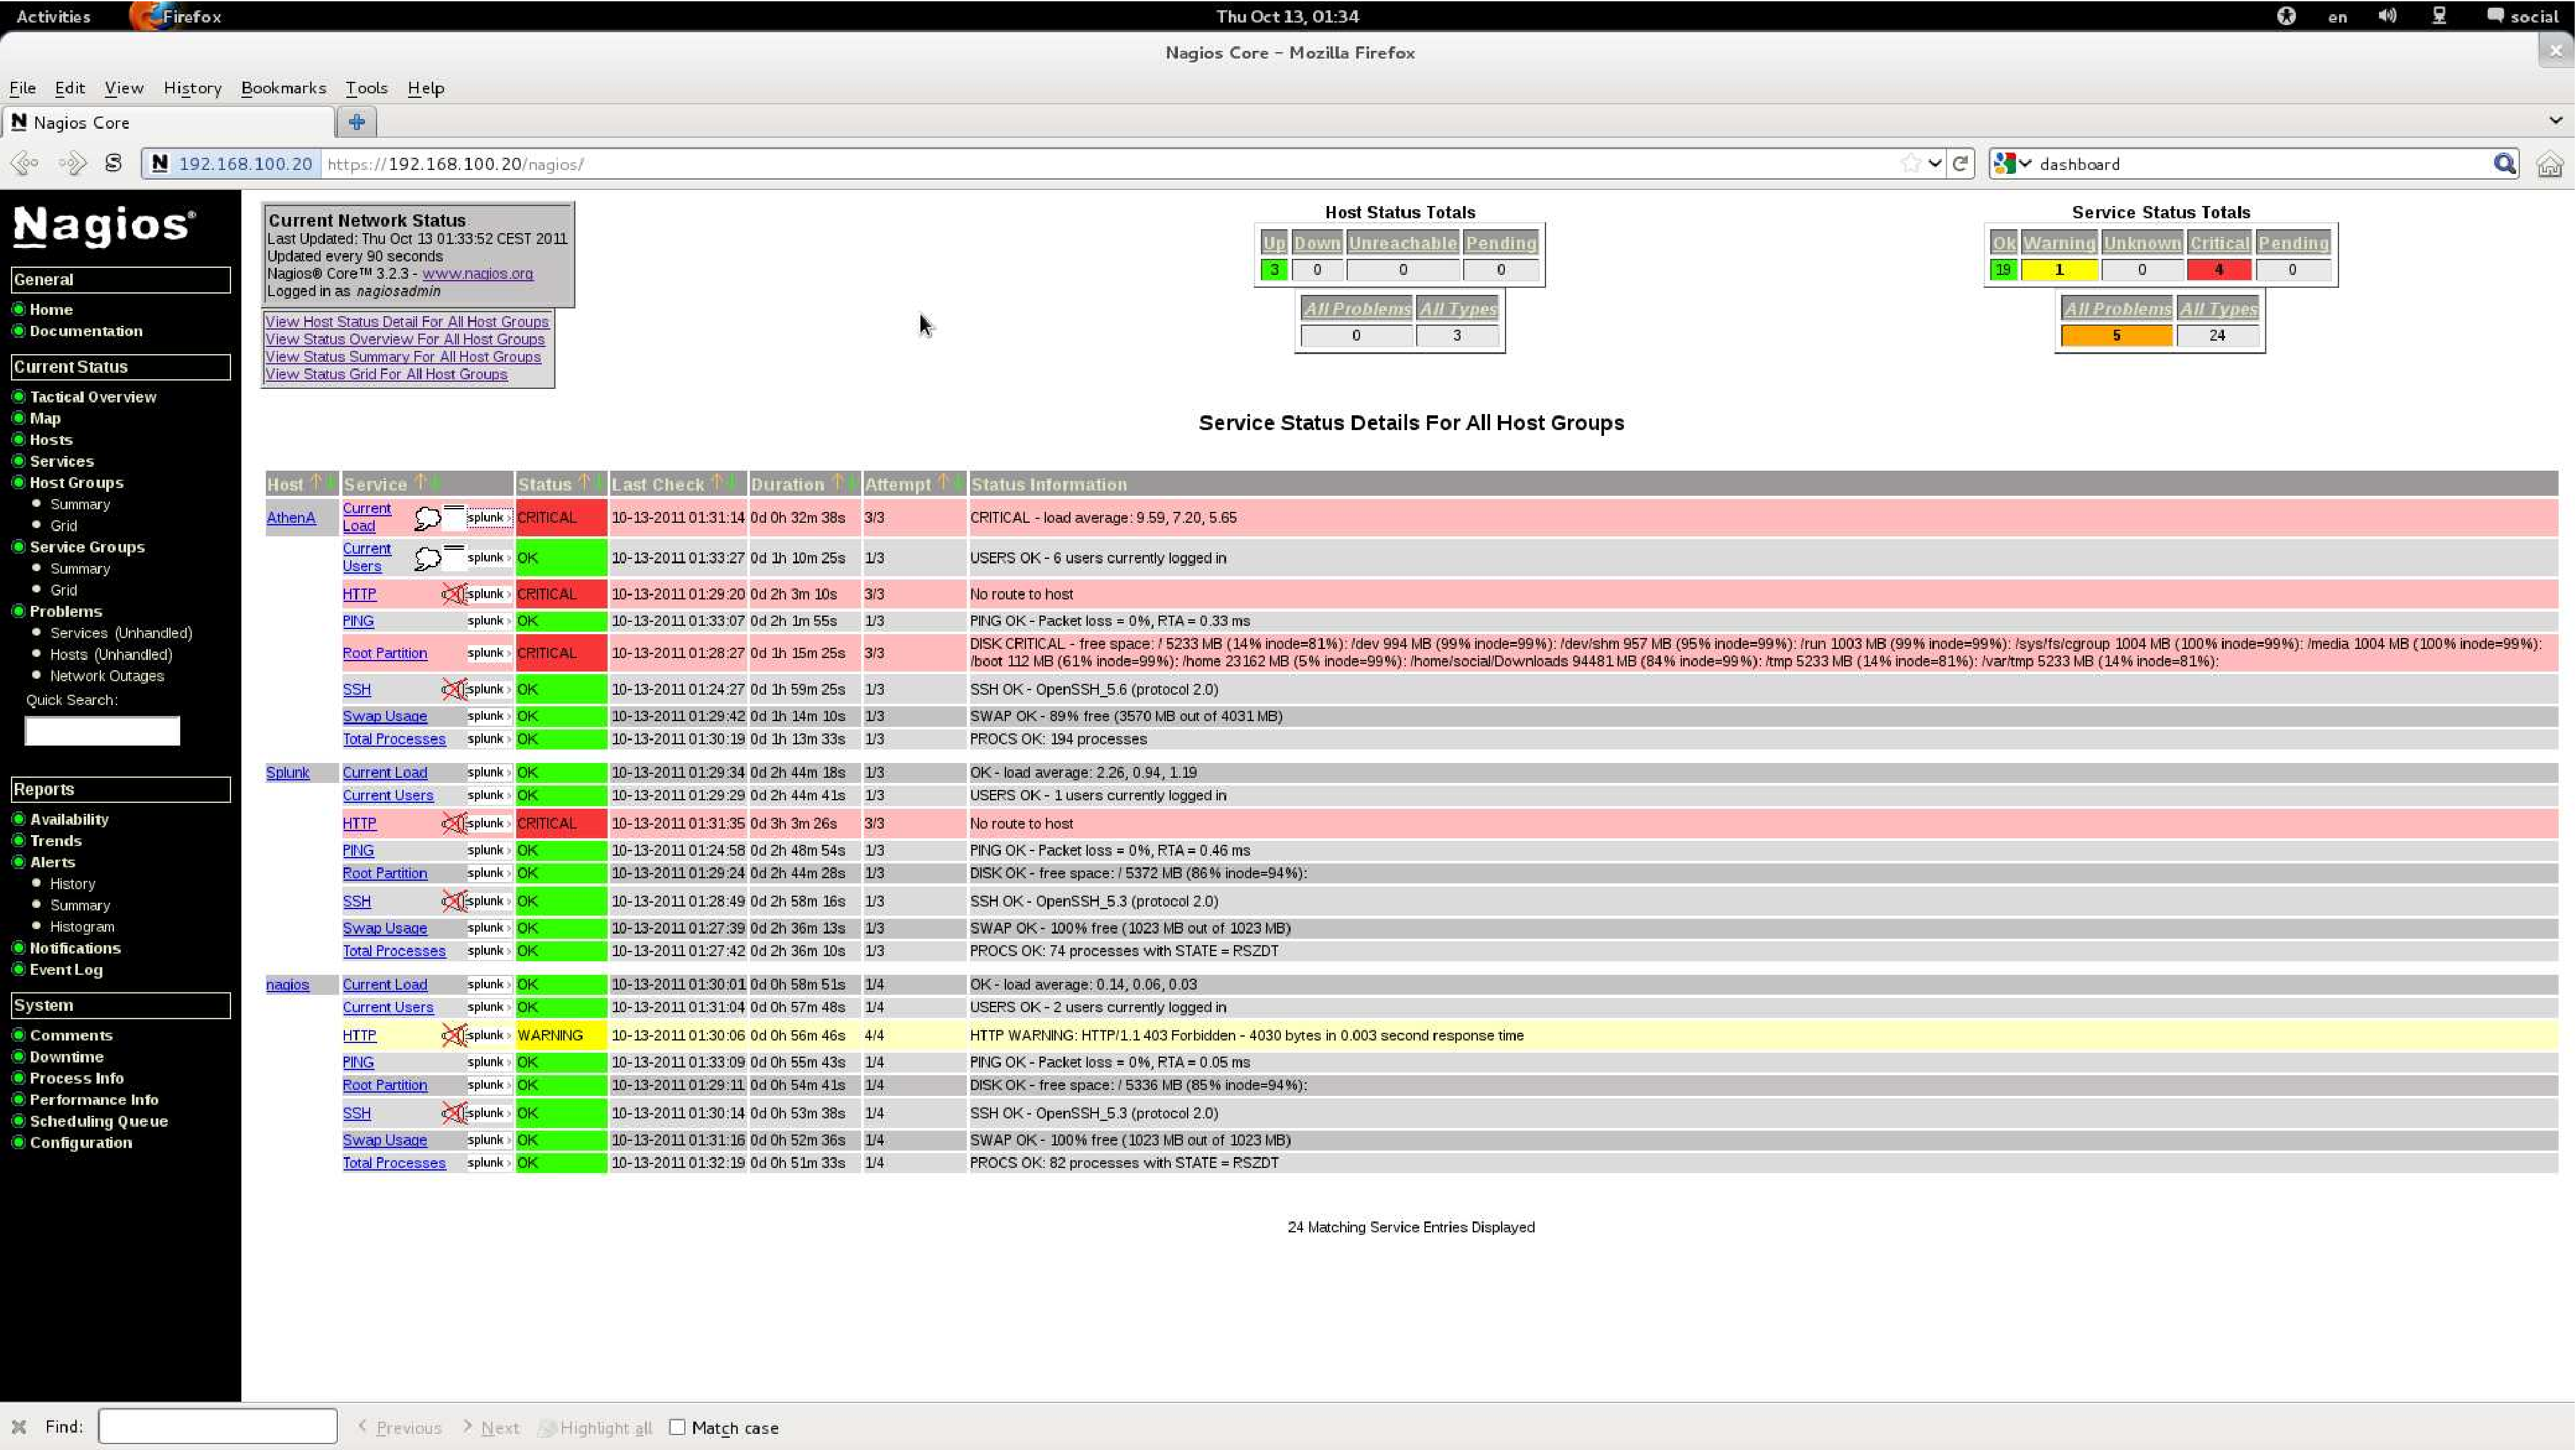
\includegraphics[width=\linewidth]{Nagios.pdf}
\end{center}
\caption{"Nagios interface.}
\label{Nagios}
\end{figure}
\begin{figure}[hbpt]
\begin{center}
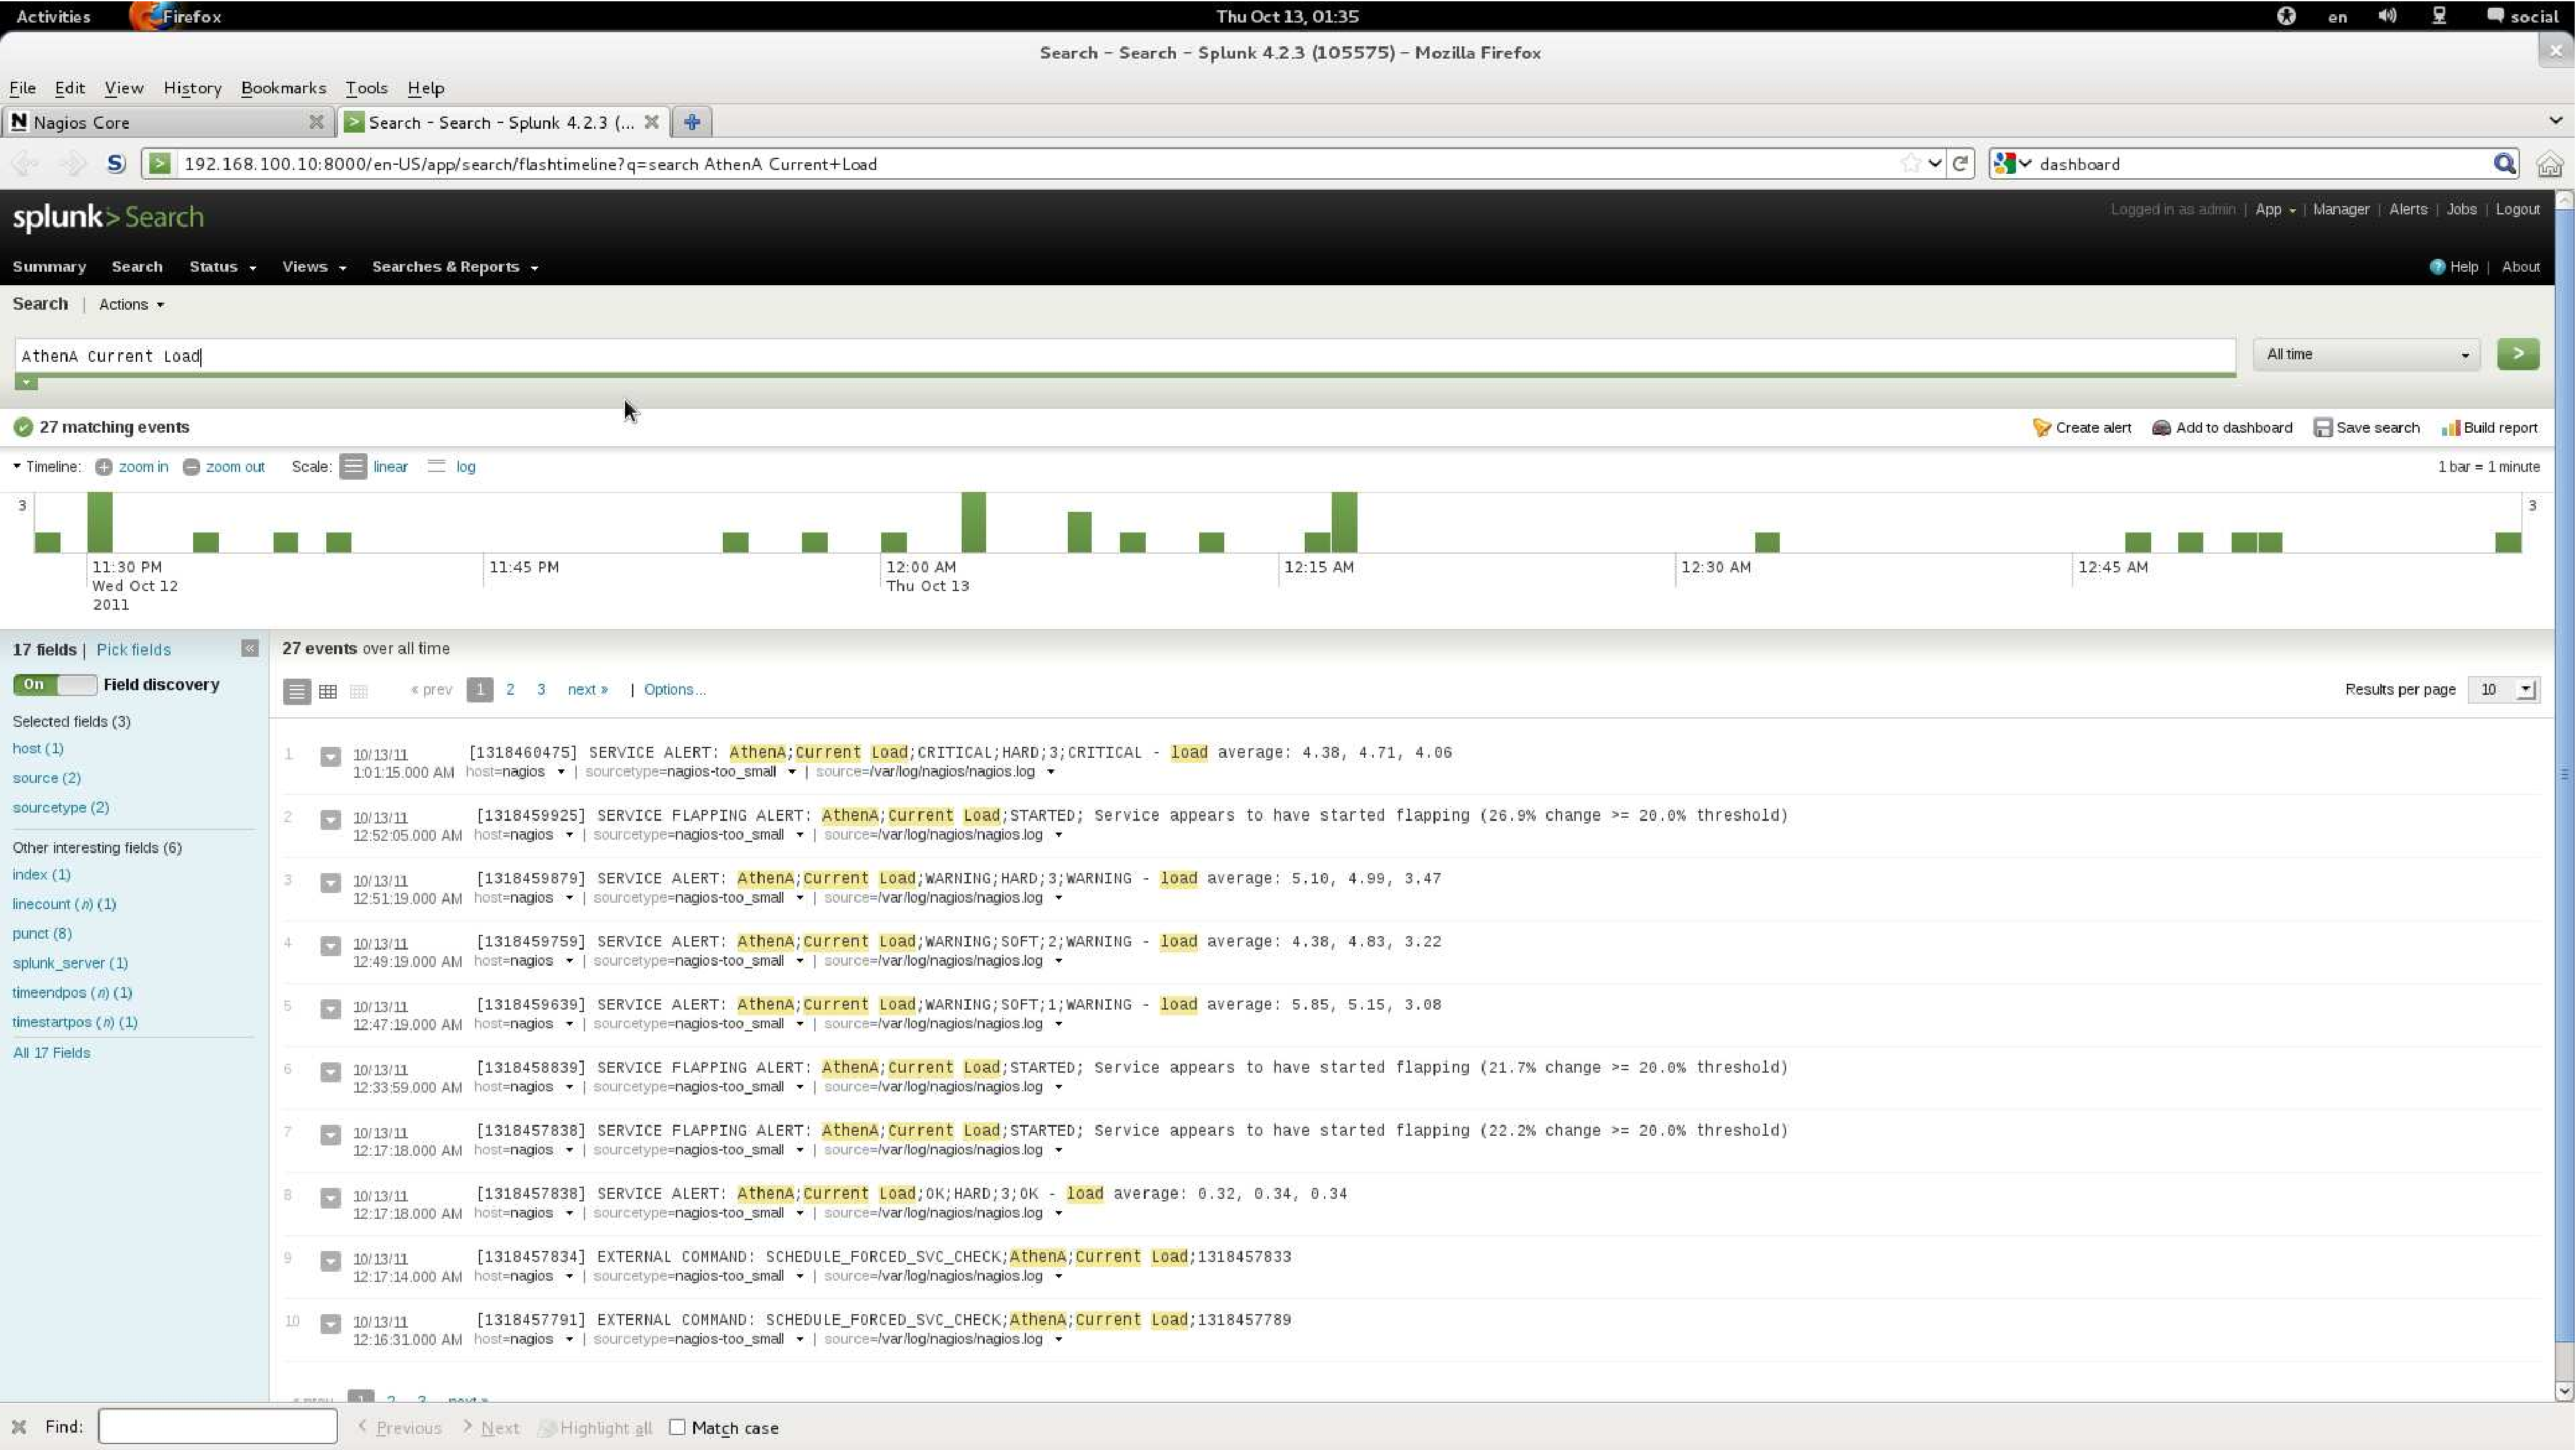
\includegraphics[width=\linewidth]{Nagios_splunk_it.pdf}
\end{center}
\caption{"Splunk it" query.}
\label{SplunkIt}
\end{figure}
\begin{figure}[hbpt]
\begin{center}
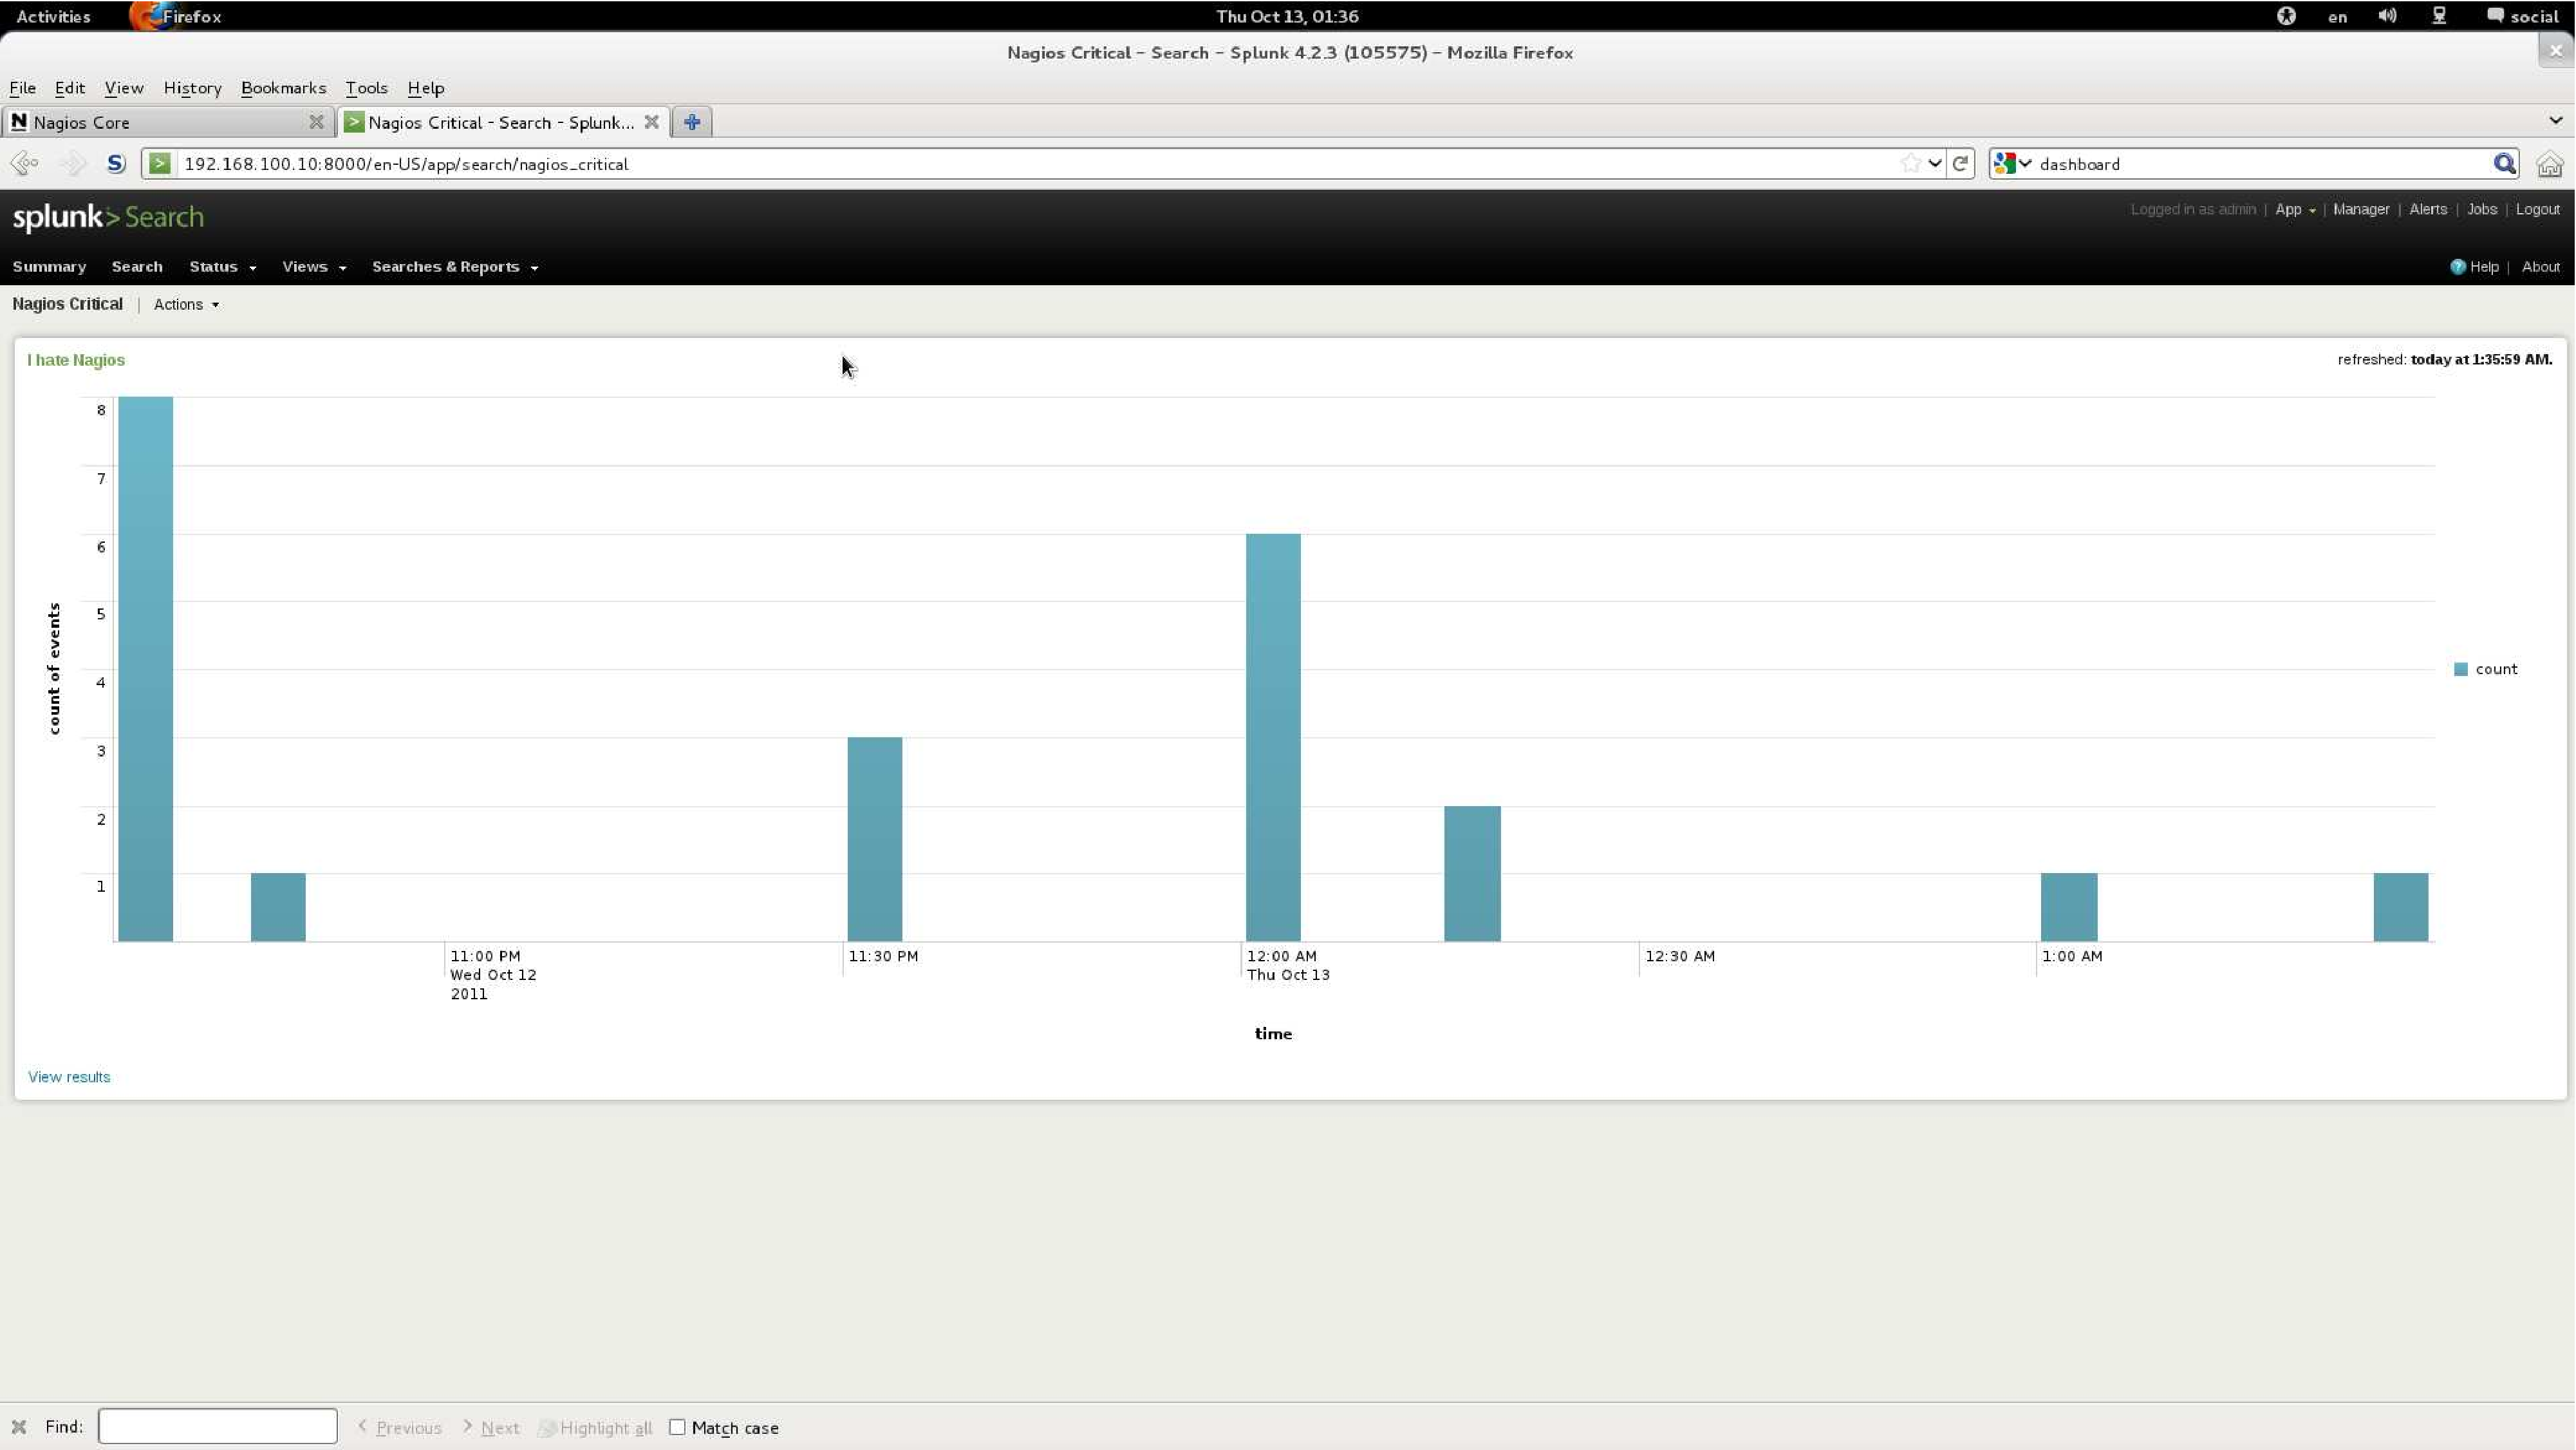
\includegraphics[width=\linewidth]{Nagios_Critical.pdf}
\end{center}
\caption{Splunk view.}
\label{report}
\end{figure}
\newpage
\appendix
%\chapter{\emph{/etc/nagios/nagios.cfg}}
\end{document}
